\section{Inertial Measurement Units}
\label{imusection}

\subsection{Introduction}

Inertial measurement units (IMU) are self-contained systems that measure linear and angular motion of an object or vehicle. Measurements are summed over a time period to determine the instantaneous position, velocity, orientation, and direction of movement.The IMU is comprised of at least two dedicated sensors, one or more linear accelerometers and one or more gyroscopes or angular accelerometers. An optional magnetometer may be integrated into the unit to calibrate against orientation drift.

\begin{figure}[!htb]
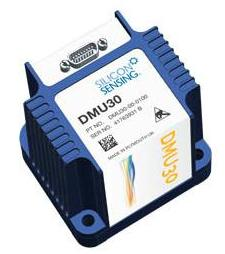
\includegraphics[width=\textwidth,height=5cm,keepaspectratio]{./figures/IMU.jpg}
\caption{IMU Physical model~\cite{StarElec}}
\label{fig:IMU Model}
\end{figure}

\subsection{Working}
IMUs operate by use of reference data, bias values from an initial starting point, and calculate changes to these values using its integrated sensors. A central processing unit calculates directional information; position, speed, orientation, and direction of movement, at a given time in space using the IMU. The sensors suffer from orientation drift as they calculate these variables using a process known as dead-reckoning and are subject to accumulative errors.Calibration parameters can be stored in the memory of an IMU and are automatically reflected in the measurement data. In-situ calibrations may also be accomplished by use of a magnetometer or GPS unit to correct for orientation drift and improve the accuracy of the directional information.
 
\begin{figure}[!htb]
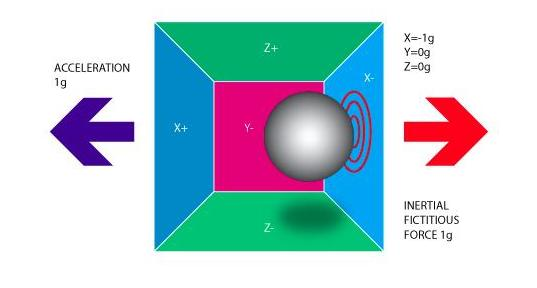
\includegraphics[width=\textwidth,height=5cm,keepaspectratio]{./figures/WorkingIMU.jpg}
\caption{Working of IMU model~\cite{StarElec}}
\label{fig:WorkingIMU}
\end{figure}

In Figure~\ref{fig:WorkingIMU}  we can see there is a weight less ball. And we are considering forward acceleration of 1 g hence ball is exerting inertial force on the box in -X direction as it is principle of action and reaction.
So here we can learn that \\

$Acceleration = \frac{force\ exerted}{mass\ of\ ball} $

Hence computing load on -X face of wall will tell us about the acceleration.
similarly if we have a ground on one side it will exert a force of g in lower direction which will be constant.
There will also be conditions where forces will be applied on two sides combined.
So its magnitude will give is the angle of tilt and accelerations in any angular directions.

So if we consider enclosed box and a ball we can measure all 3 acceleration in X,Y,Z due to all side enclosed box.
We can use sine and cosine functions to represent angles with different axis. 
So if we we take 
Angular accleration is differentiation of velocity
where\\

$Angular velocity_x= \frac{\theta_{x2} -\theta_{x1}}{T_2-T_1}$\\

So with equations and forces in all direction we can compute all 3 axis linear accelerations and all 3 angular accelerations(Gyro accelerations).